% Created 2025-01-06 Mon 06:39
% Intended LaTeX compiler: pdflatex
\documentclass[11pt,oneside]{memoir}
\makeatletter

\usepackage{answerkey-env}

\ifanswerkey
  \usepackage[forcolorpaper, answerkey]{eqexam}
  \usepackage{vinaya-class-questions}
\else
  \usepackage[forcolorpaper, nosolutions]{eqexam}
  \usepackage[nosolutions]{vinaya-class-questions}
\fi

\proofingsymbolColor{linkred}
\fillinColor{linkred}

\def\maketitle{}

\maxtocdepth{subsection}

\newenvironment{twocols}{%
  \raggedright%
  \setlength{\parindent}{0pt}%
  \setlength{\parskip}{8pt}%
  \fontsize{11}{17}\selectfont%
  \begin{multicols}{2}%
}{%
  \end{multicols}%
}

\newenvironment{widecols}{%
  \hspace*{-0.05\linewidth}\begin{minipage}{1.1\linewidth}%
  \raggedright%
  \setlength{\parindent}{0pt}%
  \setlength{\parskip}{8pt}%
  \fontsize{11}{17}\selectfont%
  \begin{multicols}{2}%
}{%
  \end{multicols}%
  \end{minipage}%
}

\newlength\@tmp@width
\newlength\@tmp@height

\renewcommand*{\printchaptertitleHook}{%
  \AddToShipoutPictureBG*{%
    \put(\LenToUnit{\paperwidth-25mm-\spinemargin},\LenToUnit{\paperheight-95mm}){%
      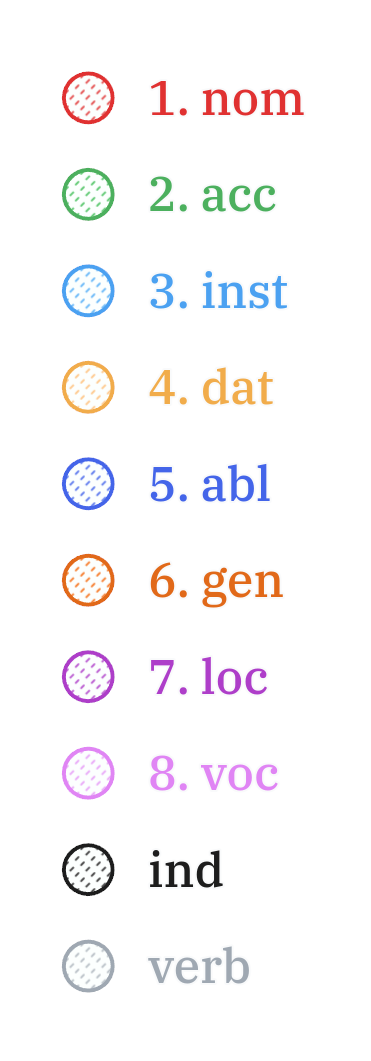
\includegraphics[width=25mm]{./images/cases-legend-white-large.png}%
    }%
  }%
}

\newcommand*\sentenceDiaMsg{\textbf{Exercise:} Draw a sentence analysis diagram below and indicate declensions.}

\newcommand*\sentenceDiaSolution[2][0.4]{%
  \ifanswerkey%
    \hspace*{-\spinemargin}%
    \begin{minipage}{\paperwidth}%
      \centering%
      \includegraphics[scale=#1]{#2}%
    \end{minipage}%
  \else%
    \settototalheight{\@tmp@height}{\includegraphics[scale=#1]{#2}}%
    \begin{minipage}[\@tmp@height]{\linewidth}%
      \sentenceDiaMsg%
    \end{minipage}%
  \fi%
}

\usepackage{cwpuzzle}

\renewcommand\PuzzleCluePre{%
  \begin{minipage}[t]{0.75\linewidth}%
}

\renewcommand\PuzzleClueFont{\fontsize{11}{17}\selectfont}

% \def\PuzzleThickline{\linethickness{2pt}}

\makeatother

\maxtocdepth{section}
\date{\today}
\title{Pāli Readings (Next)}
\hypersetup{
 pdfauthor={The Bhikkhu Saṅgha},
 pdftitle={Pāli Readings (Next)},
 pdfkeywords={},
 pdfsubject={},
 pdfcreator={Emacs 29.4 (Org mode 9.6.15)}, 
 pdflang={En_Gb}}
\begin{document}

\maketitle
\makeatletter

\newlength{\colOne}\setlength{\colOne}{0.35\linewidth}
\newlength{\colTwo}\setlength{\colTwo}{0.6\linewidth}

\renewenvironment{quote}%
{\list{}{%
    \doubleLineSize
    \listparindent 0pt
    \itemindent    0pt
    \leftmargin    3em
    \rightmargin   3em
    \parsep        0pt
    \topsep        8pt
    \partopsep     0pt}%
\item[] \raggedright}%
{\endlist}

\renewcommand*\sentenceDiaSolution[2][0.4]{%
  \ifanswerkey%
    \hspace*{-\spinemargin}%
    \begin{minipage}{\paperwidth}%
      \centering%
      \includegraphics[scale=#1]{#2}%
    \end{minipage}%
  \fi%
}

\makeatother

\mainmatter

\chapter{2025-01-08}
\label{sec:orgcb51f02}
\section{Declension Cases Overview}
\label{sec:org053b1e2}

\begin{tabular}{lll}
1. Nominative & subject performing the action & Who is giving?\\[0pt]
2. Accusative & direct object & What is he/she giving?\\[0pt]
3. Instrumental & means, instrument & With/by/through what?\\[0pt]
4. Dative & indirect object, recipient, purpose & To whom? For what?\\[0pt]
5. Ablative & motion/separation from, comparison & From where? Better than what?\\[0pt]
6. Genitive & possession, relationship & Whose?\\[0pt]
7. Locative & location, time & Where?\\[0pt]
8. Vocative & direct address & Form, bhikkhus, is not-self.\\[0pt]
\end{tabular}

\bigskip {\centering
Mnemonics:
\par}

\begin{center}
\begin{tabular}{ll}
1. \textbf{Nominate} who will do it. & 5. Pieces fall from the \textbf{ablative} heat-shield.\\[0pt]
2. Give an objective \textbf{accusation}. & 6. The \textbf{genitive} glues possessions to people.\\[0pt]
3. Fix it with this \textbf{instrument}. & 7. \textbf{Locate} him in space and time.\\[0pt]
4. \textbf{Donate} a date to him. & 8. Shout a \textbf{vocal} address.\\[0pt]
\end{tabular}
\end{center}

Origin of the word `Dative':

\begin{center}
\begin{tabular}{ll}
PIE root: & \emph{√do-} to give\\[0pt]
Latin: & \emph{donum} gift, \emph{donatio} a giving, \emph{dativus} pertaining to giving\\[0pt]
Pāli/Sanskrit: & \emph{dadāti} gives [√dā + dā + a → dadā]\\[0pt]
\end{tabular}
\end{center}

Origin of the word `Ablative':

\begin{center}
\begin{tabular}{lllll}
Latin & PIE & Pāli/Sanskrit &  & \\[0pt]
\emph{ab-} & \emph{√apo} & \emph{apa-} & off, away from & apocalypse, apology, apostle\\[0pt]
\emph{ferre} & \emph{√bher-} & \emph{√bhar} / \emph{√bhṛ} & to carry, to bear & birth, bring, burden,\\[0pt]
 &  &  &  & differ, offer, suffer, transfer\\[0pt]
\end{tabular}
\end{center}

\clearpage

\section{Cases Exercise: The Elephant}
\label{sec:orgc884e6a}

\casesLegendHeaderBGHere

\begin{quote}
Jetavane hatthinī soṇḍāya vā dīghahatthena vā

attano hatthipotakassa tiṇaṁ datvā,

tato soṇḍato mahāsaddaṁ pahiṇi.

Imassa hatthipotakassa tiṇena kucchi mahanto ahosi.
\end{quote}

\bigskip

\begin{center}
\begin{tabular}{llll}
hatthinī (f.) & female elephant [hatthī + inī] & pahiṇi (aor.) & sent; aor. of pahiṇāti\\[0pt]
soṇḍā (f.) & elephant's trunk & kucchi (m.) & stomach; belly\\[0pt]
hattha (m.) & hand & mahanta (adj.) & big; large\\[0pt]
potaka (m.) & young animal & ahosi (aor.) & was; became; aor. of hoti\\[0pt]
tiṅa (nt.) & grass; straw &  & \\[0pt]
\end{tabular}
\end{center}

\enlargethispage{\baselineskip}
\renewcommand{\arraystretch}{1.6}

\begin{center}
\begin{tabular}{lll}
word & meaning & case\\[0pt]
\hline
Jetavane & \fillin{5cm}{at Jetavana} & \fillin{3cm}{loc.}\\[0pt]
hatthinī & \fillin{5cm}{the female elephant} & \fillin{3cm}{nom.}\\[0pt]
soṇḍāya vā & \fillin{5cm}{by the trunk} & \fillin{3cm}{inst.}\\[0pt]
dīghahatthena vā & \fillin{5cm}{or by the long hand} & \fillin{3cm}{inst.}\\[0pt]
attano & \fillin{5cm}{her own} & \fillin{3cm}{gen.}\\[0pt]
hatthipotakassa & \fillin{5cm}{to the baby-elephant} & \fillin{3cm}{dat.}\\[0pt]
tiṇaṁ & \fillin{5cm}{grass} & \fillin{3cm}{acc.}\\[0pt]
datvā & \fillin{5cm}{having given} & \fillin{3cm}{ger.}\\[0pt]
tato & \fillin{5cm}{then} & \fillin{3cm}{ind.}\\[0pt]
soṇḍato & \fillin{5cm}{from the trunk} & \fillin{3cm}{abl.}\\[0pt]
mahāsaddaṁ & \fillin{5cm}{a loud noise} & \fillin{3cm}{acc.}\\[0pt]
pahiṇi & \fillin{5cm}{sent (→ pahiṇāti)} & \fillin{3cm}{aor.}\\[0pt]
imassa & \fillin{5cm}{pron. of this (→ ima)} & \fillin{3cm}{gen.sg.}\\[0pt]
hatthipotakassa & \fillin{5cm}{of the baby elephant} & \fillin{3cm}{gen.}\\[0pt]
tiṇena & \fillin{5cm}{with grass} & \fillin{3cm}{inst.}\\[0pt]
kucchi & \fillin{5cm}{belly, stomach} & \fillin{3cm}{nom.}\\[0pt]
mahanto & \fillin{5cm}{adj. great, large} & \fillin{3cm}{nom.}\\[0pt]
ahosi & \fillin{5cm}{was, became (→ hoti)} & \fillin{3cm}{aor.}\\[0pt]
\end{tabular}
\end{center}

\normalArrayStrech

\clearpage

\section{AN 10.81 Vāhanasutta, The lotus simile to Vāhana}
\label{sec:orgd6ce093}

(\href{https://suttacentral.net/an10.81/pli/ms}{SC}, \href{https://www.digitalpalireader.online/\_dprhtml/index.html?loc=a.9.0.0.1.3.0.m}{DPR}, \href{http://localhost:4848/suttas/an10.81/pli/ms?window\_type=Sutta+Study}{SSP}, Nibbāna Sermon 18)

\begin{quote}
Ekaṁ samayaṁ bhagavā campāyaṁ viharati gaggarāya pokkharaṇiyā tīre.

Atha kho āyasmā vāhano yena bhagavā tenupasaṅkami;

upasaṅkamitvā bhagavantaṁ abhivādetvā ekamantaṁ nisīdi.

Ekamantaṁ nisinno kho āyasmā vāhano bhagavantaṁ etadavoca:
\end{quote}

\begin{longtable}{L{\colOne} L{\colTwo}}
tīra (nt.) & shore, riverbank\\[0pt]
pokkhara (nt.) & blue lotus flower\\[0pt]
yena \ldots{} ten'upasaṅkamati (idiom) & wherever \ldots{} he approaches (him/it)\\[0pt]
abhivādeti & bows down (to); pays high respect (to)\\[0pt]
anta (m.) & end; side; extreme\\[0pt]
ekamantaṁ (ind.) & to one side; aside [ekaṁ + anta + aṁ]\\[0pt]
nisīdati & sits (on); sits down\\[0pt]
vacati & speaks\\[0pt]
avoca (aor. of vacati) & said (to)\\[0pt]
\end{longtable}

\begin{quote}
“Katihi nu kho, bhante, dhammehi tathāgato nissaṭo visaṁyutto vippamutto

vimariyādīkatena cetasā viharatī”ti?
\end{quote}

\begin{longtable}{L{\colOne} L{\colTwo}}
kati (interr.) & how many?\\[0pt]
nissaṭa (pp. +abl) & escaped (from), freed (from); pp. of nissarati\\[0pt]
visaṁyutta (pp. +abl) & detached (from)\\[0pt]
vippamutta (pp. +abl) & released (from)\\[0pt]
vimariyādīkata (adj.) & unbounded [vi + mariyādā + kata]\\[0pt]
mariyādā (f.) & boundary, border, limit\\[0pt]
\end{longtable}

\begin{quote}
“Dasahi kho, vāhana, dhammehi tathāgato nissaṭo visaṁyutto vippamutto vimariyādīkatena
cetasā viharati. Katamehi dasahi? Rūpena kho, vāhana, tathāgato nissaṭo visaṁyutto
vippamutto vimariyādīkatena cetasā viharati, vedanāya \ldots{} saññāya \ldots{} saṅkhārehi \ldots{} viññāṇena
\ldots{} jātiyā \ldots{} jarāya \ldots{} maraṇena \ldots{} dukkhehi \ldots{} kilesehi kho, vāhana, tathāgato nissaṭo
visaṁyutto vippamutto vimariyādīkatena cetasā viharati.
\end{quote}

\clearpage

\begin{quote}
Seyyathāpi, vāhana, uppalaṁ vā padumaṁ vā puṇḍarīkaṁ vā

udake jātaṁ udake saṁvaḍḍhaṁ udakā paccuggamma ṭhitaṁ anupalittaṁ udakena;

evamevaṁ kho, vāhana, imehi dasahi dhammehi tathāgato nissaṭo visaṁyutto

vippamutto vimariyādīkatena cetasā viharatī”ti.
\end{quote}

\begin{longtable}{L{\colOne} L{\colTwo}}
uppala, paduma, puṇḍarīka (nt.) & types of lotus\\[0pt]
udaka (nt.) & water\\[0pt]
vaḍḍhati & increases (in); grows (in)\\[0pt]
paccuggamma (ger. +abl) & going out (from), emerging (from); ger of paccuggacchati\\[0pt]
tiṭṭhati & stands\\[0pt]
anupalitta (pp. +instr) & not smeared (by), untainted (by); [na + upalitta]\\[0pt]
\end{longtable}
\end{document}
